\apendice{Documentación técnica de programación}

\section{Introducción}

En el siguiente apéndice se incluye información relevante acerca de como se encuentran estructurados los directorios que componen el proyecto, así como las instrucciones de compilación, instalación y ejecución del proyecto.

\section{Estructura de directorios}

\subsection{Estructura directorio raíz}

En el directorio raíz podemos encontrar los contenidos del proyecto agrupados conforme a los siguientes directorios:

\begin{itemize} [\textbullet]
    \item \textbf{\texttt{.github/workflows}} Contiene los ficheros correspondientes los \emph{scripts} que configuran las \textbf{GitHub Actions} del repositorio.
    \item \textbf{\texttt{/docker}} Contiene los ficheros utilizados para la configuración y compilación de los contenedores \textbf{Docker}.
    \item \textbf{\texttt{/docs}} Contiene los ficheros fuente de \LaTeX utilizados para la generación de la documentación, incluyendo las imágenes utilizadas y las versiones finales de la memoria y sus anexos.
    \item \textbf{\texttt{/prototypes}} Contiene una \textbf{prueba de concepto} de la extracción de información desde GitHub implementada en un \emph{cuaderno de \textbf{Jupyter}}, así como una serie de ficheros que contienen los datos extraídos en las pruebas.
    \item \textbf{\texttt{/scripts}} Contiene una serie de scripts tanto para Windows como para Linux que permiten medir la calidad del código mediante la realización de comprobaciones de estilo y tipado sobre el código. Son utilizados por las \textbf{GitHub Actions}.
    \item \textbf{\texttt{/src}} Contiene el código fuente del proyecto dividido en dos directorios que separan el \hyperref[mp:backend]{back-end} del \hyperref[mp:front-end]{front-end}.
\end{itemize}

\subsection{Estructura de directorios del back-end} \label{mp:backend}

\begin{itemize} [\textbullet]
    \item \textbf{\texttt{/gtmapi}} Contiene los ficheros correspondientes al servicio de API REST de la plataforma. Proporciona un acceso al sistema desde el exterior mediante el cual otras aplicaciones puedan interactuar con él.
    \item \textbf{\texttt{/gtmcore}} Contiene una serie de ficheros de utilidad requeridos para el funcionamiento del resto de servicios. Incluye la implementación de un ORM a través del cual los servicios interactúan con la base de datos.
    \item \textbf{\texttt{/gtmextraction}} Contiene los ficheros correspondientes al servicio de extracción de datos de la plataforma. Incluye las clases encargadas de establecer la conexión con GitHub.
    \item \textbf{\texttt{/gtmprocessing}} Contiene los ficheros correspondientes al servicio de procesamiento de la plataforma. Incluye la implementación de una serie de clases que permiten leer los parámetros de los experimentos, solicitar la información requerida, aplicar los modelos preentrenados y almacenar los resultados obtenidos en la base de datos.
\end{itemize}

\subsection{Estructura de directorios de la webapp} \label{mp:front-end}
Contiene todos los ficheros relacionados con la aplicación web desarrollada con el framework \textbf{React}. En esta carpeta raíz se incluye el fichero ''package.json'' que contiene las dependencias necesarias para la instalación de la web.

\begin{itemize} [\textbullet]
    \item \textbf{\texttt{/public}} Contiene una serie de ficheros relacionados con el favicon de la web.
    \item \textbf{\texttt{/src}} Contiene los ficheros de \textbf{JavaScript} que dotan a la web de sus funciones, y los ficheros \textbf{CSS} que le proporcionan su apariencia.
    \begin{itemize} [\textbullet]
        \item \textbf{\texttt{/components}} Agrupa los componentes de React desarrollados para su uso en la aplicación.
        \item \textbf{\texttt{/images}} Contiene las imágenes utilizadas en la web. 
        \item \textbf{\texttt{/pages}} Contiene las vistas de la aplicación.
        \item \textbf{\texttt{/services}} Fundamentalmente contiene los scripts necesarios para lanzar peticiones contra la API REST.
    \end{itemize}
\end{itemize}

\section{Manual del programador}

El manual del programador tiene como objetivo ayudar a comprender a los futuros programadores interesados en continuar con el desarrollo del proyecto las indicaciones necesarias para hacer uso de las llamadas contra la API REST de la aplicación, así como indicios de cómo incorporar nuevos modelos de procesamiento del lenguaje natural sobre las bases que proporciona la aplicación.

\subsection{Uso de la API REST}

En la siguiente sección se incluye un listado de los endpoint proporcionados por la API junto con los parámetros necesarios para

\subsubsection{GET - Obtener estado}

\begin{itemize} \setlength\itemsep{0.2em}
    \item[] \textbf{Respuestas}
    \begin{itemize} \setlength\itemsep{0.2em}
        \item[] \textbf{200 OK}. La aplicación se está ejecutando.
    \end{itemize}
\end{itemize}

\subsubsection{GET - Obtener listado de las tareas}

\begin{itemize}
    \item[] \textbf{Ruta}
        \begin{itemize} \setlength\itemsep{0.2em}
            \item[] \texttt{/tasks/}
        \end{itemize}
    \item[] \textbf{Respuestas}
        \begin{itemize} \setlength\itemsep{0.2em}
            \item[] \textbf{200 OK}. Se obtiene un objeto JSON con un único atributo \textit{eqlts} que contiene un listado de objetos tarea.
                \begin{itemize} \setlength\itemsep{0.2em}
                    \item[] \textbf{Content-Type}: \texttt{application/json/}.
                    \item[] \textbf{Body}: 
                        \begin{itemize}
                            \item[] \textbf{task\_id}: Number
                            \item[] \textbf{state}: Number
                            \item[] \textbf{timestamp}: String
                            \item[] \textbf{repo\_dir}: String
                            \item[] \textbf{task\_type}: Number
                            \item[] \textbf{params}: Object
                        \end{itemize}
                \end{itemize}
            \item[] \textbf{500 Internal Server error}. Se ha producido un error interno en la aplicación.
        \end{itemize}
\end{itemize}

\subsubsection{GET - Obtener listado de los repositorios}

\begin{itemize}
    \item[] \textbf{Ruta}
        \begin{itemize} \setlength\itemsep{0.2em}
            \item[] \texttt{/repos/}
        \end{itemize}
    \item[] \textbf{Respuestas}
        \begin{itemize} \setlength\itemsep{0.2em}
            \item[] \textbf{200 OK}. Se obtiene un objeto JSON con un único atributo \textit{eqlts} que contiene un listado de objetos respositorio.
                \begin{itemize} \setlength\itemsep{0.2em}
                    \item[] \textbf{Content-Type}: \texttt{application/json/}.
                    \item[] \textbf{Body}: 
                        \begin{itemize} \setlength\itemsep{0.2em}
                            \item[] \textbf{repo\_dir}: String
                            \item[] \textbf{title}: String
                            \item[] \textbf{description}: String
                            \item[] \textbf{labels}: List
                        \end{itemize}
                \end{itemize}
            \item[] \textbf{500 Internal Server error}. Se ha producido un error interno en la aplicación.
        \end{itemize}
\end{itemize}

\subsubsection{GET - Obtener listado de las incidencias}

\begin{itemize}
    \item[] \textbf{Ruta}
        \begin{itemize} \setlength\itemsep{0.2em}
            \item[] \texttt{/issues/}
        \end{itemize}
    \item[] \textbf{Respuestas}
        \begin{itemize} \setlength\itemsep{0.2em}
            \item[] \textbf{200 OK}. Se obtiene un objeto JSON con un único atributo \textit{eqlts} que contiene un listado de objetos incidencia.
                \begin{itemize} \setlength\itemsep{0.2em}
                    \item[] \textbf{Content-Type}: \texttt{application/json/}.
                    \item[] \textbf{Body}: 
                        \begin{itemize} \setlength\itemsep{0.2em}
                            \item[] \textbf{repo\_dir}: String
                            \item[] \textbf{issue\_id}: Number
                            \item[] \textbf{author}: String
                            \item[] \textbf{title}: String
                            \item[] \textbf{description}: String
                            \item[] \textbf{labels}: List
                            \item[] \textbf{is\_pull\_request}: Boolean
                        \end{itemize}
                \end{itemize}
            \item[] \textbf{500 Internal Server error}. Se ha producido un error interno en la aplicación.
        \end{itemize}
\end{itemize}

\subsubsection{GET - Obtener listado de los comentarios}

\begin{itemize}
    \item[] \textbf{Ruta}
        \begin{itemize} \setlength\itemsep{0.2em}
            \item[] \texttt{/comments/}
        \end{itemize}
    \item[] \textbf{Respuestas}
        \begin{itemize} \setlength\itemsep{0.2em}
            \item[] \textbf{200 OK}. Se obtiene un objeto JSON con un único atributo \textit{eqlts} que contiene un listado de objetos comentario.
                \begin{itemize} \setlength\itemsep{0.2em}
                    \item[] \textbf{Content-Type}: \texttt{application/json/}.
                    \item[] \textbf{Body}: 
                        \begin{itemize} \setlength\itemsep{0.2em}
                            \item[] \textbf{repo\_dir}: String
                            \item[] \textbf{issue\_id}: Number
                            \item[] \textbf{comment\_id}: Number
                            \item[] \textbf{author}: String
                            \item[] \textbf{body}: String
                        \end{itemize}
                \end{itemize}
            \item[] \textbf{500 Internal Server error}. Se ha producido un error interno en la aplicación.
        \end{itemize}
\end{itemize}

\subsubsection{GET - Obtener listado de los resultados de las ejecuciones}

\begin{itemize}
    \item[] \textbf{Ruta}
        \begin{itemize} \setlength\itemsep{0.2em}
            \item[] \texttt{/outcomes/}
        \end{itemize}
    \item[] \textbf{Respuestas}
        \begin{itemize} \setlength\itemsep{0.2em}
            \item[] \textbf{200 OK}. Se obtiene un objeto JSON con un único atributo \textit{eqlts} que contiene un listado de objetos resultado.
                \begin{itemize} \setlength\itemsep{0.2em}
                    \item[] \textbf{Content-Type}: \texttt{application/json/}.
                    \item[] \textbf{Body}: 
                        \begin{itemize} \setlength\itemsep{0.2em}
                            \item[] \textbf{task\_id}: Number
                            \item[] \textbf{repo\_dir}: String
                            \item[] \textbf{model\_type}: String
                            \item[] \textbf{outcome\_data}: JSON
                            \item[] \textbf{exec\_time}: Number
                        \end{itemize}
                \end{itemize}
            \item[] \textbf{500 Internal Server error}. Se ha producido un error interno en la aplicación.
        \end{itemize}
\end{itemize}

\subsubsection{POST - Extraer la información de un repositorio}

\begin{itemize}
    \item[] \textbf{Ruta}
        \begin{itemize} \setlength\itemsep{0.2em}
            \item[] \texttt{/extract/}
        \end{itemize}
    \item[] \textbf{Parámetros}
        \begin{itemize} \setlength\itemsep{0.2em}
            \item[] \textbf{Content-Type}: \texttt{application/json/}.
            \item[] \textbf{Body}: 
                \begin{itemize} \setlength\itemsep{0.2em}
                    \item[] \textbf{gh\_user}: String
                    \item[] \textbf{gh\_repo}: String
                \end{itemize}
        \end{itemize}
    \item[] \textbf{Respuestas}
        \begin{itemize} \setlength\itemsep{0.2em}
            \item[] \textbf{200 OK}. Se obtiene un objeto JSON con un indicador de que la tarea ha sido encolada correctamente y su identificador único.
                \begin{itemize} \setlength\itemsep{0.2em}
                    \item[] \textbf{Content-Type}: \texttt{application/json/}.
                    \item[] \textbf{Body}: 
                        \begin{itemize} \setlength\itemsep{0.2em}
                            \item[] \textbf{Added}: [Body] Boolean
                            \item[] \textbf{task\_id}: [Body] Number
                        \end{itemize}
                \end{itemize}
            \item[] \textbf{400 Bad Request}. Los parámetros introducidos son incorrectos.
            \item[] \textbf{500 Internal Server error}. Se ha producido un error interno en la aplicación.
        \end{itemize}
\end{itemize}

\subsubsection{GET - Obtener la información de un repositorio}

\begin{itemize}
    \item[] \textbf{Ruta}
        \begin{itemize} \setlength\itemsep{0.2em}
            \item[] \texttt{/user/<string:gh\_user>/repo/<string:gh\_repo>}
        \end{itemize}
    \item[] \textbf{Parámetros}
        \begin{itemize} \setlength\itemsep{0.2em}
            \item[] \textbf{gh\_user}: [Path] String
            \item[] \textbf{gh\_repo}: [Path] String
        \end{itemize}
    \item[] \textbf{Respuestas}
        \begin{itemize} \setlength\itemsep{0.2em}
            \item[] \textbf{200 OK}. Se obtiene un objeto JSON con la información del repositorio.
                \begin{itemize} \setlength\itemsep{0.2em}
                    \item[] \textbf{Content-Type}: \texttt{application/json/}.
                    \item[] \textbf{Body}: 
                        \begin{itemize} \setlength\itemsep{0.2em}
                            \item[] \textbf{repo\_dir}: String
                            \item[] \textbf{title}: String
                            \item[] \textbf{description}: String
                            \item[] \textbf{labels}: List
                        \end{itemize}
                \end{itemize}
            \item[] \textbf{202 Accepted}. La petición es correcta pero la información solicitada aún no se encuentra disponible.
            \item[] \textbf{404 Not Found}. No se encuentra ningún repositorio de acuerdo con los parámetros introducidos.
            \item[] \textbf{424 Failed Dependency}. La extracción de los datos del repositorio falló.
            \item[] \textbf{500 Internal Server error}. Se ha producido un error interno en la aplicación.
        \end{itemize}
\end{itemize}

\subsubsection{GET - Obtener la información de una incidencia de un repositorio}

\begin{itemize}
    \item[] \textbf{Ruta}
        \begin{itemize} \setlength\itemsep{0.2em}
            \item[] \texttt{/user/<string:gh\_user>/repo/<string:gh\_repo>/issue/<int:issue\_id>}
        \end{itemize}
    \item[] \textbf{Parámetros}
        \begin{itemize} \setlength\itemsep{0.2em}
            \item[] \textbf{gh\_user}: [Path] String
            \item[] \textbf{gh\_repo}: [Path] String
            \item[] \textbf{issue\_id}: [Path] Number            
        \end{itemize}
    \item[] \textbf{Respuestas}
        \begin{itemize} \setlength\itemsep{0.2em}
            \item[] \textbf{200 OK}. Se obtiene un objeto JSON con la información de la incidencia.
                \begin{itemize} \setlength\itemsep{0.2em}
                    \item[] \textbf{Content-Type}: \texttt{application/json/}.
                    \item[] \textbf{Body}: 
                        \begin{itemize} \setlength\itemsep{0.2em}
                            \item[] \textbf{repo\_dir}: String
                            \item[] \textbf{issue\_id}: Number
                            \item[] \textbf{author}: String
                            \item[] \textbf{title}: String
                            \item[] \textbf{description}: String
                            \item[] \textbf{labels}: List
                            \item[] \textbf{is\_pull\_request}: Boolean
                        \end{itemize}
                \end{itemize}
            \item[] \textbf{400 Bad Request}. Los parámetros introducidos son incorrectos.
            \item[] \textbf{404 Not Found}. No se encuentra ninguna incidencia de acuerdo con los parámetros introducidos.
            \item[] \textbf{500 Internal Server error}. Se ha producido un error interno en la aplicación.
        \end{itemize}
\end{itemize}

\subsubsection{GET - Obtener las incidencias de un repositorio}

\begin{itemize}
    \item[] \textbf{Ruta}
        \begin{itemize} \setlength\itemsep{0.2em}
            \item[] \texttt{/user/<string:gh\_user>/repo/<string:gh\_repo>/issues}
        \end{itemize}
    \item[] \textbf{Parámetros}
        \begin{itemize} \setlength\itemsep{0.2em}
            \item[] \textbf{gh\_user}: [Path] String
            \item[] \textbf{gh\_repo}: [Path] String
        \end{itemize}
    \item[] \textbf{Respuestas}
        \begin{itemize} \setlength\itemsep{0.2em}
            \item[] \textbf{200 OK}. Se obtiene un objeto JSON con una lista incidencias del repositorio.
                \begin{itemize} \setlength\itemsep{0.2em}
                    \item[] \textbf{Content-Type}: \texttt{application/json/}.
                    \item[] \textbf{Body}: 
                        \begin{itemize} \setlength\itemsep{0.2em}
                            \item[] \textbf{repo\_dir}: String
                            \item[] \textbf{issue\_id}: Number
                            \item[] \textbf{author}: String
                            \item[] \textbf{title}: String
                            \item[] \textbf{description}: String
                            \item[] \textbf{labels}: List
                            \item[] \textbf{is\_pull\_request}: Boolean
                        \end{itemize}
                \end{itemize}
            \item[] \textbf{202 Accepted}. La petición es correcta pero la información solicitada aún no se encuentra disponible.
            \item[] \textbf{404 Not Found}. No se encuentra ningún repositorio de acuerdo con los parámetros introducidos.
            \item[] \textbf{424 Failed Dependency}. La extracción de los datos del repositorio falló.
            \item[] \textbf{500 Internal Server error}. Se ha producido un error interno en la aplicación.
        \end{itemize}
\end{itemize}

\subsubsection{GET - Obtener los comentarios de una incidencia}

\begin{itemize}
    \item[] \textbf{Ruta}
        \begin{itemize} \setlength\itemsep{0.2em}
            \item[] \texttt{/user/<string:gh\_user>/repo/<string:gh\_repo>/issue/<int:issue\_id>/comments}
        \end{itemize}
    \item[] \textbf{Parámetros}
        \begin{itemize} \setlength\itemsep{0.2em}
            \item[] \textbf{gh\_user}: [Path] String
            \item[] \textbf{gh\_repo}: [Path] String
            \item[] \textbf{issue\_id}: [Path] Number
        \end{itemize}
    \item[] \textbf{Respuestas}
        \begin{itemize} \setlength\itemsep{0.2em}
            \item[] \textbf{200 OK}. Se obtiene un objeto JSON con una lista comentarios de la incidencia.
                \begin{itemize} \setlength\itemsep{0.2em}
                    \item[] \textbf{Content-Type}: \texttt{application/json/}.
                    \item[] \textbf{Body}: 
                        \begin{itemize} \setlength\itemsep{0.2em}
                            \item[] \textbf{repo\_dir}: String
                            \item[] \textbf{issue\_id}: Number
                            \item[] \textbf{author}: String
                            \item[] \textbf{title}: String
                            \item[] \textbf{description}: String
                            \item[] \textbf{labels}: List
                            \item[] \textbf{is\_pull\_request}: Boolean
                        \end{itemize}
                \end{itemize}
            \item[] \textbf{202 Accepted}. La petición es correcta pero la información solicitada aún no se encuentra disponible.
            \item[] \textbf{404 Not Found}. No se encuentra ningún repositorio de acuerdo con los parámetros introducidos.
            \item[] \textbf{424 Failed Dependency}. La extracción de los datos del repositorio falló.
            \item[] \textbf{500 Internal Server error}. Se ha producido un error interno en la aplicación.
        \end{itemize}
\end{itemize}

\subsubsection{GET - Obtener las operaciones realizadas sobre un repositorio}

\begin{itemize}
    \item[] \textbf{Ruta}
        \begin{itemize} \setlength\itemsep{0.2em}
            \item[] \texttt{/user/<string:gh\_user>/repo/<string:gh\_repo>/tasks}
        \end{itemize}
    \item[] \textbf{Parámetros}
        \begin{itemize} \setlength\itemsep{0.2em}
            \item[] \textbf{gh\_user}: [Path] String
            \item[] \textbf{gh\_repo}: [Path] String
        \end{itemize}
    \item[] \textbf{Respuestas}
        \begin{itemize} \setlength\itemsep{0.2em}
            \item[] \textbf{200 OK}. Se obtiene un objeto JSON con la lista de las operaciones realizadas sobre el repositorio.
                \begin{itemize} \setlength\itemsep{0.2em}
                    \item[] \textbf{Content-Type}: \texttt{application/json/}.
                    \item[] \textbf{Body}: 
                        \begin{itemize} \setlength\itemsep{0.2em}
                            \item[] \textbf{task\_id}: Number
                            \item[] \textbf{state}: Number
                            \item[] \textbf{timestamp}: String
                            \item[] \textbf{repo\_dir}: String
                            \item[] \textbf{task\_type}: Number
                            \item[] \textbf{params}: Object
                        \end{itemize}
                \end{itemize}
            \item[] \textbf{204 No Content}. No se localizan registros de repositorios que concuerden con los parámetros introducidos.
            \item[] \textbf{500 Internal Server error}. Se ha producido un error interno en la aplicación.
        \end{itemize}
\end{itemize}

\subsubsection{GET - Obtener los experimentos lanzados sobre un repositorio}

\begin{itemize}
    \item[] \textbf{Ruta}
        \begin{itemize} \setlength\itemsep{0.2em}
            \item[] \texttt{/user/<string:gh\_user>/repo/<string:gh\_repo>/experiments}
        \end{itemize}
    \item[] \textbf{Parámetros}
        \begin{itemize} \setlength\itemsep{0.2em}
            \item[] \textbf{gh\_user}: [Path] String
            \item[] \textbf{gh\_repo}: [Path] String
        \end{itemize}
    \item[] \textbf{Respuestas}
        \begin{itemize} \setlength\itemsep{0.2em}
            \item[] \textbf{200 OK}. Se obtiene un objeto JSON con la lista de los resultados de los experimentos lanzados sobre el repositorio.
                \begin{itemize} \setlength\itemsep{0.2em}
                    \item[] \textbf{Content-Type}: \texttt{application/json/}.
                    \item[] \textbf{Body}: 
                        \begin{itemize} \setlength\itemsep{0.2em}
                            \item[] \textbf{task\_id}: Number
                            \item[] \textbf{repo\_dir}: String
                            \item[] \textbf{model\_type}: String
                            \item[] \textbf{outcome\_data}: JSON
                            \item[] \textbf{exec\_time}: Number
                        \end{itemize}
                \end{itemize}
            \item[] \textbf{204 No Content}. No se localizan registros de repositorios que concuerden con los parámetros introducidos.
            \item[] \textbf{500 Internal Server error}. Se ha producido un error interno en la aplicación.
        \end{itemize}
\end{itemize}

\subsubsection{POST - Lanzar un experimento de Zero-Shot Classification sobre un repositorio}

\begin{itemize}
    \item[] \textbf{Ruta}
        \begin{itemize} \setlength\itemsep{0.2em}
            \item[] \texttt{/user/<string:gh\_user>/repo/<string:gh\_repo>/process/zsc/}
        \end{itemize}
    \item[] \textbf{Content-Type}: \texttt{application/json/}.
    \item[] \textbf{Parámetros}
        \begin{itemize} \setlength\itemsep{0.2em}
            \item[] \textbf{gh\_user}: [Path] String
            \item[] \textbf{gh\_repo}: [Path] String
            \item[] \textbf{issue\_id}: [Body] Number
            \item[] \textbf{accuracy}: [Body] Float. Entre 0 y 1.
            \item[] \textbf{use\_desc}: [Body] Boolean
            \item[] \textbf{extra\_labels}: [Body] String. Cada término deberá estar separado por un punto y coma.
        \end{itemize}
    \item[] \textbf{Respuestas}
        \begin{itemize} \setlength\itemsep{0.2em}
            \item[] \textbf{200 OK}. Se obtiene un objeto JSON con un indicador de que el experimento ha sido encolado correctamente y su identificador único.
                \begin{itemize} \setlength\itemsep{0.2em}
                    \item[] \textbf{Content-Type}: \texttt{application/json/}.
                    \item[] \textbf{Body}: 
                        \begin{itemize} \setlength\itemsep{0.2em}
                            \item[] \textbf{Added}: [Body] Boolean
                            \item[] \textbf{task\_id}: [Body] Number
                        \end{itemize}
                \end{itemize}
            \item[] \textbf{400 Bad Request}. Los parámetros introducidos son incorrectos.
            \item[] \textbf{406 Not Acceptable}. Los parámetros introducidos no se corresponden con ninguno de los repositorios disponibles.
            \item[] \textbf{500 Internal Server error}. Se ha producido un error interno en la aplicación.
            \item[] \textbf{503 Service Unavailable}. En estos momentos no es posible lanzar el experimento sobre el repositorio solicitado.
        \end{itemize}
\end{itemize}

\subsubsection{POST - Lanzar un experimento de Sentiment Analysis sobre un repositorio}

\begin{itemize}
    \item[] \textbf{Ruta}
        \begin{itemize} \setlength\itemsep{0.2em}
            \item[] \texttt{/user/<string:gh\_user>/repo/<string:gh\_repo>/process/sa/}
        \end{itemize}
    \item[] \textbf{Content-Type}: \texttt{application/json/}.
    \item[] \textbf{Parámetros}
        \begin{itemize} \setlength\itemsep{0.2em}
            \item[] \textbf{gh\_user}: [Path] String
            \item[] \textbf{gh\_repo}: [Path] String
            \item[] \textbf{issue\_id}: [Body] Integer
            \item[] \textbf{author}: [Body] String.
            \item[] \textbf{with\_comments}: [Body] Boolean
        \end{itemize}
    \item[] \textbf{Respuestas}
        \begin{itemize} \setlength\itemsep{0.2em}
            \item[] \textbf{200 OK}. Se obtiene un objeto JSON con un indicador de que el experimento ha sido encolado correctamente y su identificador único.
                \begin{itemize} \setlength\itemsep{0.2em}
                    \item[] \textbf{Content-Type}: \texttt{application/json/}.
                    \item[] \textbf{Body}: 
                        \begin{itemize} \setlength\itemsep{0.2em}
                            \item[] \textbf{Added}: [Body] Boolean
                            \item[] \textbf{task\_id}: [Body] Number
                        \end{itemize}
                \end{itemize}
            \item[] \textbf{400 Bad Request}. Los parámetros introducidos son incorrectos.
            \item[] \textbf{406 Not Acceptable}. Los parámetros introducidos no se corresponden con ninguno de los repositorios disponibles.
            \item[] \textbf{500 Internal Server error}. Se ha producido un error interno en la aplicación.
            \item[] \textbf{503 Service Unavailable}. En estos momentos no es posible lanzar el experimento sobre el repositorio solicitado.
        \end{itemize}
\end{itemize}

\subsubsection{POST - Lanzar un experimento de Summarization sobre un repositorio}

\begin{itemize}
    \item[] \textbf{Ruta}
        \begin{itemize} \setlength\itemsep{0.2em}
            \item[] \texttt{/user/<string:gh\_user>/repo/<string:gh\_repo>/process/summ/}
        \end{itemize}
    \item[] \textbf{Content-Type}: \texttt{application/json/}.
    \item[] \textbf{Parámetros}
        \begin{itemize} \setlength\itemsep{0.2em}
            \item[] \textbf{gh\_user}: [Path] String
            \item[] \textbf{gh\_repo}: [Path] String
            \item[] \textbf{max\_length}: [Body] Integer
            \item[] \textbf{min\_length}: [Body] Integer
            \item[] \textbf{with\_comments}: [Body] Boolean
        \end{itemize}
    \item[] \textbf{Respuestas}
        \begin{itemize} \setlength\itemsep{0.2em}
            \item[] \textbf{200 OK}. Se obtiene un objeto JSON con un indicador de que el experimento ha sido encolado correctamente y su identificador único.
                \begin{itemize} \setlength\itemsep{0.2em}
                    \item[] \textbf{Content-Type}: \texttt{application/json/}.
                    \item[] \textbf{Body}: 
                        \begin{itemize} \setlength\itemsep{0.2em}
                            \item[] \textbf{Added}: [Body] Boolean
                            \item[] \textbf{task\_id}: [Body] Number
                        \end{itemize}
                \end{itemize}
            \item[] \textbf{400 Bad Request}. Los parámetros introducidos son incorrectos.
            \item[] \textbf{406 Not Acceptable}. Los parámetros introducidos no se corresponden con ninguno de los repositorios disponibles.
            \item[] \textbf{500 Internal Server error}. Se ha producido un error interno en la aplicación.
            \item[] \textbf{503 Service Unavailable}. En estos momentos no es posible lanzar el experimento sobre el repositorio solicitado.
        \end{itemize}
\end{itemize}

\section{Instalación y ejecución del proyecto}

En el siguiente apartado se presentan las instrucciones a través de las cuales establecer un entorno de desarrollo que disponga del código fuente, utilidades, complementos y ejecutables requeridos para la puesta en marcha del proyecto. 

\subsection{Prerrequisitos}
El código fuente del proyecto se ha implementado haciendo uso de los lenguajes de programación \textbf{Python} y \textbf{JavaScript}. En el caso de Python este se requiere para las implementaciones llevadas a cabo en el apartado del front-end. El uso de JavaScript se debe al desarrollo de la aplicación web, implementada sobre el entorno de ejecución \textbf{NodeJS}. A continuación se incluyen las versiones requeridas por la aplicación para asegurar su correcto funcionamiento:
\begin{itemize}
    \item \textbf{Python 3.9.6} o superior.
    \item \textbf{NodeJS 14.17.4} o superior.
    \item \textbf{Docker 20.10.12} o superior.
    \item \textbf{Docker Compose 1.29.2} o superior.
\end{itemize}
Se recomienda el uso del editor de texto \textbf{Visual Studio Code} debido a la versatilidad que ofrece a la hora de trabajar con diversos lenguajes de manera simultánea y el uso de extensiones que facilitan múltiples aspectos en el proceso de desarrollo.

\subsection{Obtención el proyecto}

El proyecto se encuentra alojado en un repositorio de GitHub de acceso libre. Para proceder con la obtención de una copia local de los ficheros se recurrirá a un software de control de versiones que ofrezcan soporte a repositorios de GitHub como \textbf{Git} o \textbf{GitHub Desktop}. También es posible la descarga directa de los ficheros a través de la dirección de GitHub en la cual se encuentra alojado el repositorio. La dirección de acceso al repositorio es la siguiente:

\vspace{0.5cm}
\centerline{\texttt{\url{https://github.com/MrpYA45/github-text-mining-tfg}}}
\vspace{0.4cm}

En caso de que se haya decidido escoger el popular software de control de versiones Git el comando requerido para la obtención de los archivos es el siguiente:

\vspace{0.5cm}
\centerline{\texttt{git clone https://github.com/MrpYA45/github-text-mining-tfg}}
\vspace{0.4cm}

\begin{figure}[!ht]
	\centering
    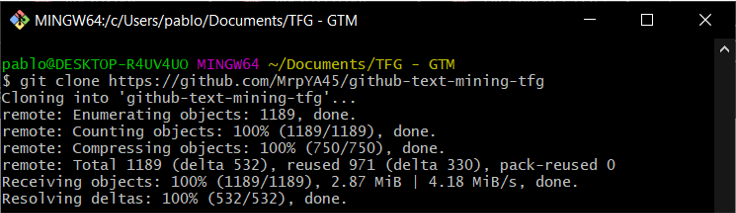
\includegraphics[width=\textwidth]{img/git_gtm.png}
	\caption{Obtención del repositorio mediante Git.}
	\label{fig:git_gtm_mp}
\end{figure}

\subsection{Preparación de un entorno virtual}

Los entornos virtuales de Python permiten mantener varios desarrollos en el mismo equipo de manera que las configuraciones y dependencias de un entorno se mantengan aisladas del resto de entornos virtuales. No es un requisito obligatorio su uso pero sí recomendable para evitar conflictos entre posibles múltiples versiones de las dependencias utilizadas entre proyectos, manteniendo solo aquellas estrictamente necesarias para el desarrollo. 

Para crear un entorno virtual se deberá situar la terminal en el directorio raíz del proyecto y ejecutar el comando dispuesto a continuación:

\vspace{0.5cm}
\centerline{\textbf{MacOS/Linux:} \texttt{python3 -m venv env}}
\centerline{\textbf{Windows:} \texttt{python -m venv env}}
\vspace{0.4cm}

\begin{figure}[!ht]
	\centering
    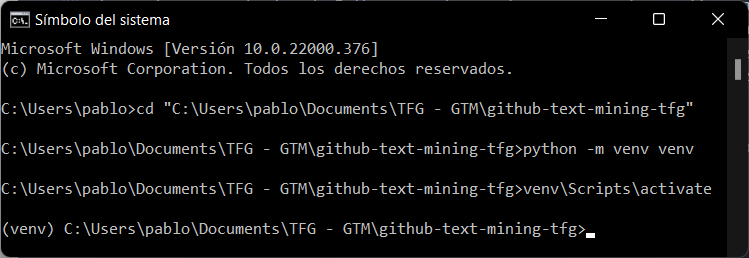
\includegraphics[width=\textwidth]{img/creating_venv.png}
	\caption{Creación de un entorno virtual para Python.}
	\label{fig:python_venv_creation}
\end{figure}

Una vez se disponga de un entorno virtual deberemos activarlo, para la cual el comando a utilizar dependerá del sistema operativo que se vaya a utilizar (véase \autoref{fig:python_venv_creation}).

\vspace{0.5cm}
\centerline{\textbf{MacOS/Linux:} \texttt{source venv/bin/activate}}
\centerline{\textbf{Windows:} \texttt{venv\textbackslash Scripts\textbackslash activate}}
\vspace{0.4cm}

\subsection{Instalación de las dependencias del back-end}
Seguidamente se realizará la instalación de las dependencias de Python utilizadas en el proyecto de acuerdo con el listado de paquetes que se proporciona en el directorio raíz del proyecto mediante el fichero \texttt{requirements.txt}. La instalación se realizará a través del gestor de paquetes \textbf{PIP}, el cual se distribuye junto con Python desde la versión 3.4.

\vspace{0.5cm}
\centerline{\textbf{MacOS/Linux:} \texttt{pip3 install -r requirements.txt}}
\centerline{\textbf{Windows:} \texttt{pip install -r requirements.txt}}
\vspace{0.4cm}

\subsection{Instalación de las dependencias de la aplicación web}
A continuación, se procederá con la instalación de las dependencias de la aplicación web. Esta se encuentra construida sobre el entorno de ejecución NodeJS basado en JavaScript. La aplicación web también ha sido desarrollada haciendo uso de módulos que simplifican la programación de ciertos aspectos de la web.

Para proceder a la instalación de estas dependencias se deberá situar la terminal en la carpeta \texttt{src/webapp}. El fichero \texttt{package.json} es el encargado de almacenar el listado con las dependencias necesarias para poder proceder con la instalación, así como los \textit{scripts} que permiten lanzar la aplicación. Para proceder con la instalación de los ficheros necesarios se deberá recurrir al siguiente comando:

\vspace{0.5cm}
\centerline{\textbf{Windows/MacOS/Linux: } \texttt{npm install}}
\vspace{0.4cm}

\subsection{Lanzamiento de los servicios del back-end}

El lanzamiento de los servicios del back-end se realizará por medio del uso de las herramientas \textbf{Docker} y \textbf{Docker Compose}, para las cuales se ha diseñado una configuración que permite mantener cada uno de los servicios y la base de datos en contenedores independientes.

El primer paso consistirá en la obtención de las imágenes que se ejecutarán en el interior de los contenedores. Para ello, situándonos en la directorio raíz del proyecto, se deberá ejecutar el comando de construcción que se incluye a continuación. Se ha de tener en cuenta que la primera ejecución del comando requiere de la descarga de numerosos archivos pesados, por ello por lo que el proceso puede alargarse durante varios minutos.

\vspace{0.5cm}
\centerline{\textbf{Windows/MacOS/Linux:}}
\centerline{\texttt{docker-compose -f docker/config/docker-compose.yml build}}
\vspace{0.4cm}

Una vez se ha completado el proceso de generación de las imágenes se deberá proseguir con el levantamiento de los contenedores que contendrán dichas imágenes. En una primera instancia este proceso requiere de un extenso tiempo de espera durante el cual se procede a la descarga e instalación de las dependencias requeridas por los servicios en el interior de los propios contenedores.

\vspace{0.5cm}
\centerline{\textbf{Windows/MacOS/Linux:}}
\centerline{\texttt{docker-compose -f docker/config/docker-compose.yml up}}
\vspace{0.4cm}

El servicio con un mayor tiempo de despliegue inicial resulta ser el servicio de procesamiento denominado \textit{gtmprocessing}, el cual puede llegar a requerir de entre 10 y 15 minutos en su arranque. Ante la pobre vivacidad que se presenta en el proceso de obtención de los modelos se recomienda realizar comprobaciones periódicas a través del siguiente comando.

\vspace{0.5cm}
\centerline{\textbf{Windows/MacOS/Linux: } \texttt{docker logs gtmprocessing -t}}
\vspace{0.4cm}

Esta orden permite obtener un visualizar la actividad que se está produciendo en el interior del contenedor. A través de esta salida se podrá comprobar el estado de la descarga de los modelos.

\subsubsection{Configuración inicial de los servicios}

Una vez finalizado el proceso de configuración inicial se deberá verificar que se han generado correctamente los ficheros de configuración. Estos ficheros se encuentran en el interior de cada uno de los servicios en la ruta \texttt{/src/backend/\%service\_name\%/config}.

Verificada la existencia de estos ficheros se deberán detener los contenedores para poder proceder a su pertinente configuración.

\vspace{0.5cm}
\centerline{\textbf{Windows/MacOS/Linux:}}
\centerline{\texttt{docker-compose -f docker/config/docker-compose.yml stop}}
\vspace{0.4cm}

Cada servicio dispone de una carpeta \textit{gtmcore} en su configuración que permite alterar los parámetros de conexión con la base de datos. Por defecto, estos ficheros se generan con una configuración básica de acuerdo con la configuración de la base de datos establecida en el fichero de variables de entorno de Docker localizado en la siguiente ruta \texttt{docker/services/.env}. Se recomienda encarecidamente modificar estos valores en caso de lanzar la aplicación en algún entorno de producción.

Finalmente, el servicio de extracción dispone de una segunda carpeta de configuración denominada \textit{gtmprocessing}. En su interior se encuentra un fichero de configuración que se requiere completar para lograr la extracción de la información de los repositorios. Este fichero solicita un token de acceso personal de GitHub.

Una vez se haya completado la configuración de los servicios se deberá volver a levantar los contenedores con el comando señalado anteriormente. En el momento en que los servicios se encuentren completamente desplegados será posible acceder a la API REST de la aplicación por medio de consultas a la dirección \url{http://localhost:6060/}.

\subsubsection{Obtención de un token de acceso personal de GitHub}

La obtención de un token de acceso personal de GitHub requiere de encontrarnos registrados en la plataforma. Una vez en ella se puede solicitar el token desde el apartado de \textit{Settings}, \textit{Developer Settings}, y seleccionar el apartado \href{https://github.com/settings/tokens}{\textit{Personal Access Tokens}}.

La generación de un token requiere del establecimiento de un periodo de caducidad y de la selección de una serie de permisos básicos para poder realizar ciertas acciones. El uso básico de las peticiones que se realizan por parte de la aplicación implica que solo se requiere del permiso de acceso a repositorios públicos (véase \autoref{fig:gen_github_access_tokens_mp}).

\begin{figure}[!ht]
	\centering
    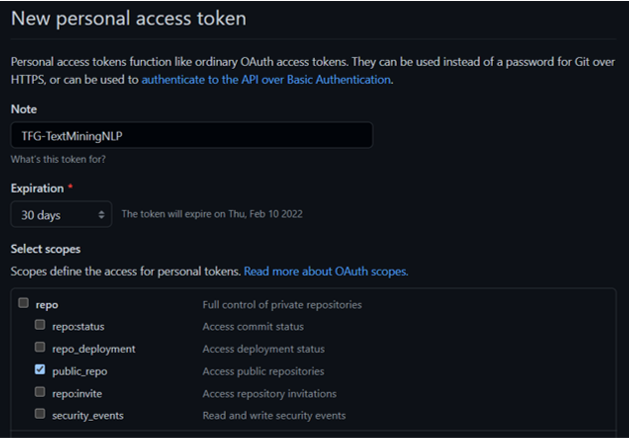
\includegraphics[width=\textwidth]{img/gen_github_access_tokens.png}
	\caption{Generación del Token de Acceso Personal en GitHub.}
	\label{fig:gen_github_access_tokens_mp}
\end{figure}

\subsection{Lanzamiento de la aplicación web mediante NodeJS}

El lanzamiento de aplicación web solamente requiere de la situación de la terminal en la ruta donde se localiza los ficheros de la aplicación web (\texttt{src/webapp}) y la introducción del siguiente comando. 

\vspace{0.5cm}
\centerline{\textbf{Windows/MacOS/Linux: } \texttt{npm start gtm-webapp}}
\vspace{0.4cm}

Tras su ejecución se producirá el despliegue de la aplicación en un servidor de NodeJS y la apertura automática de una ventana en el navegador web presentando al usuario la web. En caso de que esto no suceda por algún motivo desconocido, la aplicación web se encuentra accesible desde la siguiente dirección \url{http://localhost:3000/}.

\section{Pruebas del sistema}

Las pruebas de sistema permiten comprobar la robustez de este mediante el sometimiento del sistema a métricas o situaciones que verifiquen la respuesta de este ciertas condiciones cumpliendo con los requisitos establecidos. Durante el desarrollo del proyecto se destaca el uso de dos tipos de pruebas: pruebas de calidad de código y pruebas de comportamiento. 

\subsection{Métricas de calidad de código y documentación}

La verificación de la calidad del código se ha llevado a cabo a partir del uso de las herramientas \textbf{Pylint} y \textbf{MyPy} de Python cuyo objetivo consiste en comprobar que el código se adapta unos estándares de calidad adecuados. Ambas herramientas han sido utilizadas por medio de ficheros ejecutables que se encuentran accesibles en la carpeta \textit{scripts} del proyecto.

El paquete Pylint se encarga de comprobar y verificar que el código y su documentación se adapta a la guía de estilo \textbf{PEP 8} (Python Enhancement Proposal 8). Las comprobaciones realizadas por esta herramienta se basan en calificar multitud de escenarios y dotar al proyecto de una puntuación de acuerdo con dichas métricas de calidad.

El paquete MyPy tiene como objetivo comprobar que se hace un buen uso de los tipos estáticos recientemente introducidos en Python por medio de anotaciones. La utilización de este tipo de técnicas de programación facilita la depuración y localización de errores en un lenguaje tan dinámico como este.

\subsection{Pruebas de comportamiento de la API REST}

La comprobación del comportamiento y resolución de los \textit{endpoints} de la API REST han sido llevadas a cabo por medio del uso de la herramienta Postman. Para verificar que los puntos de acceso se mantuvieran accesibles y respondiesen de acuerdo con los requisitos se ha generado una colección de pruebas que permitiría conocer y revisar su comportamiento (véase \autoref{fig:postman_rest_testing}).

\begin{figure}[!ht]
	\centering
    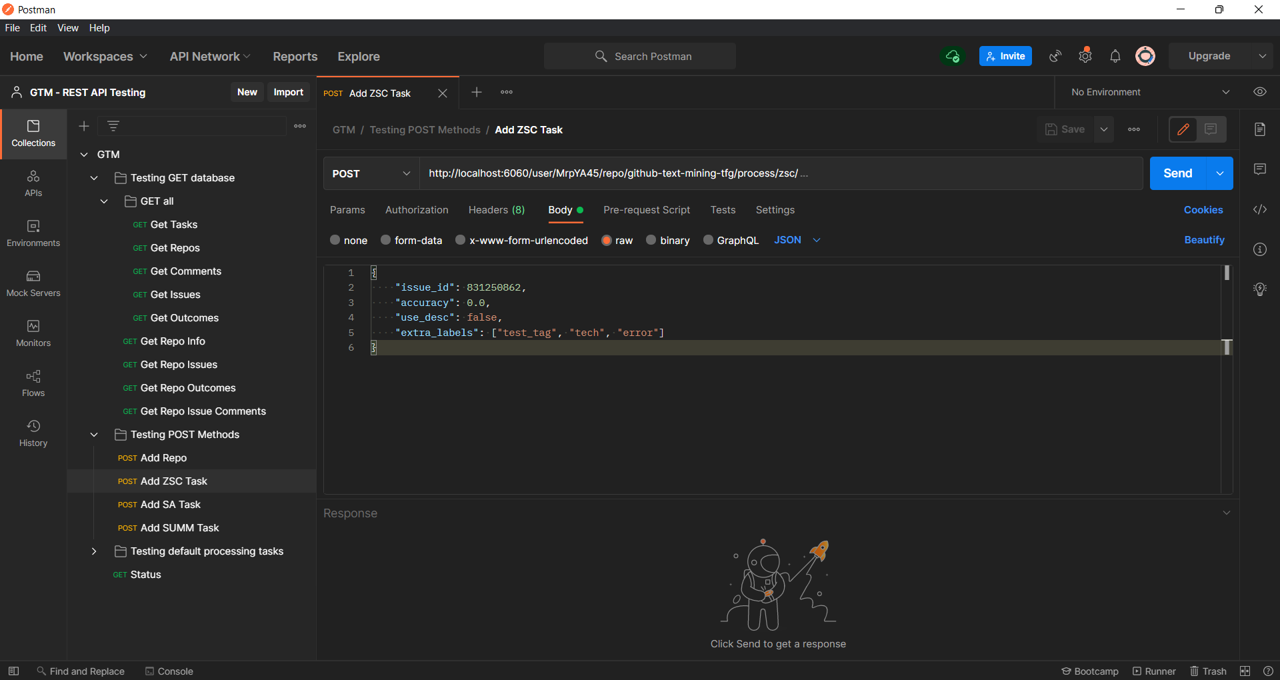
\includegraphics[width=\textwidth]{img/postman_rest_testing.png}
	\caption{Colección de pruebas de comportamiento en Postman.}
	\label{fig:postman_rest_testing}
\end{figure}